% ============================ Part 2: Language modeling ============================
\section{Part 2 $\cdot$ Language modeling}
\partslide{2}{Language modeling}{predicting the next token}

\begin{frame}{A language model assigns probabilities to text}
\begin{itemize}\setlength{\itemsep}{6pt}
  \item A \textbf{language model (LM)} assigns a probability to any sequence of tokens $x_1, \dots, x_T$.
  \item Chain rule of probability:
  \[
    P(x_1,\dots,x_T) \;=\; \prod_{t=1}^{T} P(x_t \mid x_{<t})
  \]
  \item Example: \; $P(\text{I eat the apple}) = P(\text{I})\cdot P(\text{eat}\mid\text{I})\cdot P(\text{the}\mid\text{I eat})\cdot P(\text{apple}\mid\text{I eat the})$
\end{itemize}
\vspace{8pt}
\keybox{So an LM only ever has to answer \textbf{one} question, over and over:\\[3pt] \centering\emph{given the text so far, what comes next?} \quad $P(x_t \mid x_{<t})$}
\end{frame}

\begin{frame}{Two ways to estimate $P(x_t \mid x_{<t})$}
\begin{columns}[T]
\begin{column}{0.6\textwidth}
\textbf{Old way: count ($n$-gram models)}
{\small
\begin{align*}
  P(\text{apple}\mid \text{I eat the}) &= \frac{P(\text{I eat the apple})}{P(\text{I eat the})} && \text{\scriptsize\color{midgray} conditional probability}\\[2pt]
  &\approx \frac{\#(\text{I eat the apple})}{\#(\text{I eat the})} && \text{\scriptsize\color{midgray} count in a corpus}
\end{align*}}
\vspace{-4pt}
\begin{itemize}\setlength{\itemsep}{3pt}
  \item each probability $\approx$ (count)/(corpus size); the corpus size cancels
  \item most 4-word sequences never occur, even in a huge corpus
  \item fixed window, no generalization
\end{itemize}
\end{column}
\begin{column}{0.38\textwidth}
\textbf{New way: a neural network}
\[
  P(x_t \mid x_{<t}) \approx \mathrm{NN}_\theta(x_{<t})
\]
\begin{itemize}\setlength{\itemsep}{3pt}
  \item learns continuous representations; generalizes to unseen phrasings
  \item can condition on thousands of previous tokens
\end{itemize}
\end{column}
\end{columns}
\vspace{10pt}
\callback{this course}{A network with parameters $\theta$, trained by gradient descent on a loss --- same as every model since Lecture 2.}
\end{frame}

\begin{frame}{The simplest neural language model}
\begin{center}
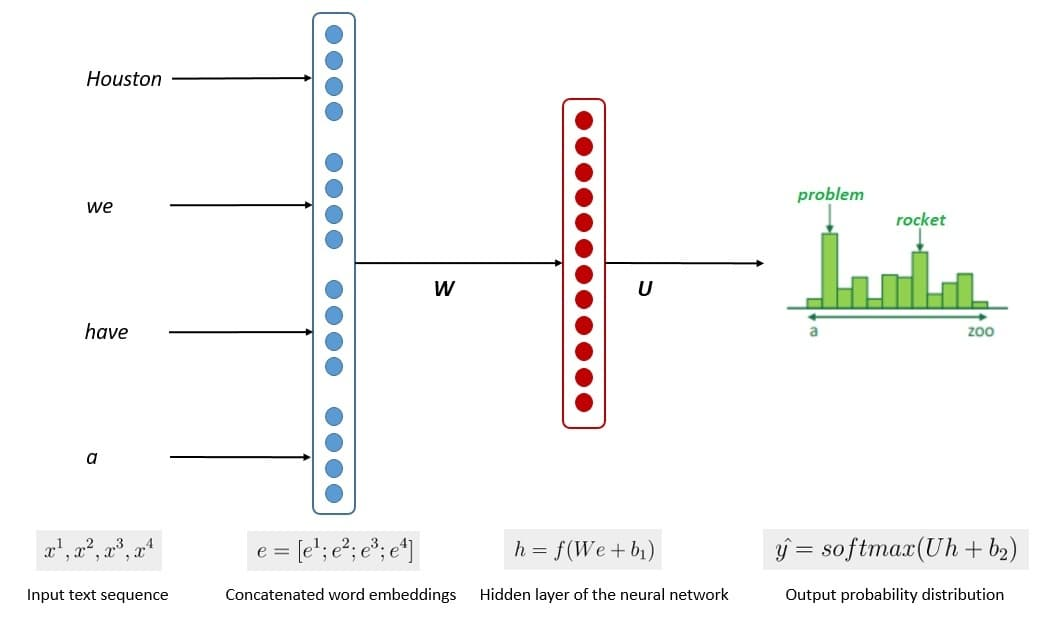
\includegraphics[width=0.66\textwidth]{figs/ffnn_lm.png}
\end{center}
\vspace{-2pt}
\begin{itemize}\setlength{\itemsep}{3pt}
  \item Look up an \textbf{embedding} for each of the last few tokens and concatenate them; one \textbf{hidden layer}; a \textbf{softmax} over the whole vocabulary.
  \item This is the feed-forward network you already know, with a $|V|$-way output. Modern LLMs swap the middle for a Transformer and keep both ends.
\end{itemize}
\end{frame}

\begin{frame}{Step 0: tokenization --- text becomes a sequence of integers}
\begin{columns}[T]
\begin{column}{0.52\textwidth}
\begin{itemize}\setlength{\itemsep}{5pt}
  \item A \textbf{token} is a common chunk of characters; the \textbf{vocabulary} $V$ lists all tokens ($|V|\approx$ 50k--128k).
  \item \textbf{Tokenization} maps text $\to$ token IDs in $\{1,\dots,|V|\}$.
  \item \textbf{Subword} tokens: frequent words are one token, rare words are split:\\ \quad \texttt{unhappiness} $\to$ \texttt{un} + \texttt{happi} + \texttt{ness}
  \item \gray{Foreshadowing: the model never sees letters, only tokens --- one reason ``how many r's in \emph{strawberry}'' is hard (Part 3).}
\end{itemize}
\end{column}
\begin{column}{0.46\textwidth}
\centering
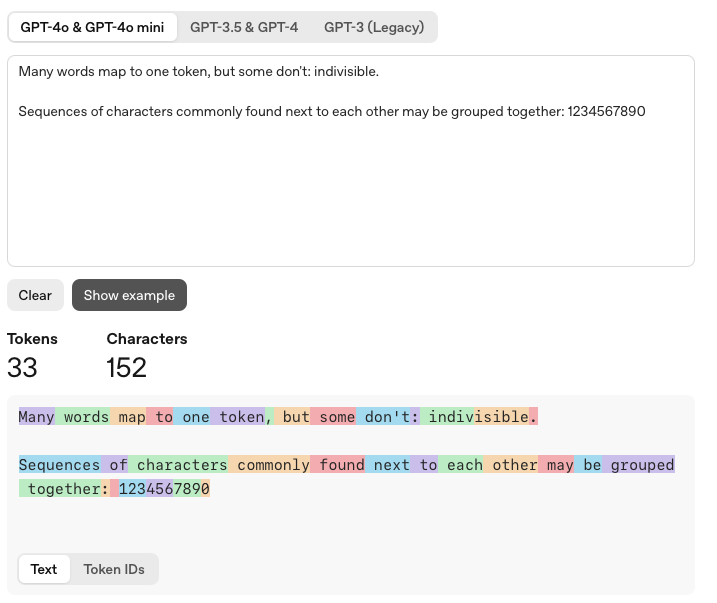
\includegraphics[width=0.95\textwidth]{figs/tokenizer_screenshot.png}\\
\scriptsize 152 characters $\to$ 33 tokens. \url{https://platform.openai.com/tokenizer}
\end{column}
\end{columns}
\end{frame}

\begin{frame}{The whole model, end to end}
\begin{center}
\begin{tikzpicture}[font=\scriptsize,>=Latex,node distance=3.3mm,
  box/.style={draw,rounded corners,minimum height=1.3cm,minimum width=1.38cm,align=center,thick},
  tok/.style={draw,rounded corners,fill=white,minimum width=0.85cm,inner sep=2pt}]
  \node[tok] (t1) {I}; \node[tok,below=1mm of t1] (t2) {eat}; \node[tok,below=1mm of t2] (t3) {the};
  \node[box,fill=uvaorange!15,draw=uvaorange!80!black,right=5mm of t2] (tk) {Tokenization\\\tiny text $\to$ IDs};
  \node[box,fill=uvaorange!15,draw=uvaorange!80!black,right=of tk] (em) {Embedding\\\tiny ID $\to$ $e_t\in\mathbb{R}^d$};
  \node[box,fill=uvanavy!12,draw=uvanavy,right=of em] (nn) {Neural\\network $f_\theta$\\\tiny a Transformer};
  \node[box,fill=okgreen!12,draw=okgreen!70!black,right=of nn] (lg) {Logits\\\tiny $z_t\in\mathbb{R}^{|V|}$};
  \node[box,fill=okgreen!12,draw=okgreen!70!black,right=of lg] (sm) {Softmax\\\tiny probabilities $p_t$};
  \node[box,fill=okgreen!12,draw=okgreen!70!black,right=of sm] (dc) {Decoding\\\tiny pick a token};
  \node[tok,right=5mm of dc] (out) {apple};
  \draw[->,thick] (t2) -- (tk); \draw[->,thick] (tk) -- (em); \draw[->,thick] (em) -- (nn);
  \draw[->,thick] (nn) -- (lg); \draw[->,thick] (lg) -- (sm); \draw[->,thick] (sm) -- (dc); \draw[->,thick] (dc) -- (out);
  \draw[->,thick,dashed,gray] (out.south) |- ++(0,-0.75) -| node[pos=0.25,below,font=\tiny]{append and repeat} (t3.south);
  \node[below=0.9cm of sm,text=okgreen!70!black,font=\scriptsize\itshape,xshift=0.6cm,align=center] {you already know\\this part};
\end{tikzpicture}
\end{center}
\vspace{4pt}
\begin{itemize}\setlength{\itemsep}{4pt}
  \item \textbf{Embedding:} a learned lookup table $E\in\mathbb{R}^{|V|\times d}$; token ID $i_t$ becomes the vector $e_t = E_{i_t}$.
  \item \textbf{Network:} a deep neural network (a Transformer) turns $e_1,\dots,e_t$ into one vector $h_t\in\mathbb{R}^d$ that summarizes ``the text so far''.
  \item \textbf{Head:} a linear layer + softmax turns $h_t$ into a distribution over the next token.
\end{itemize}
\end{frame}

\begin{frame}{The network is a Transformer}
\begin{columns}[T]
\begin{column}{0.4\textwidth}
\centering
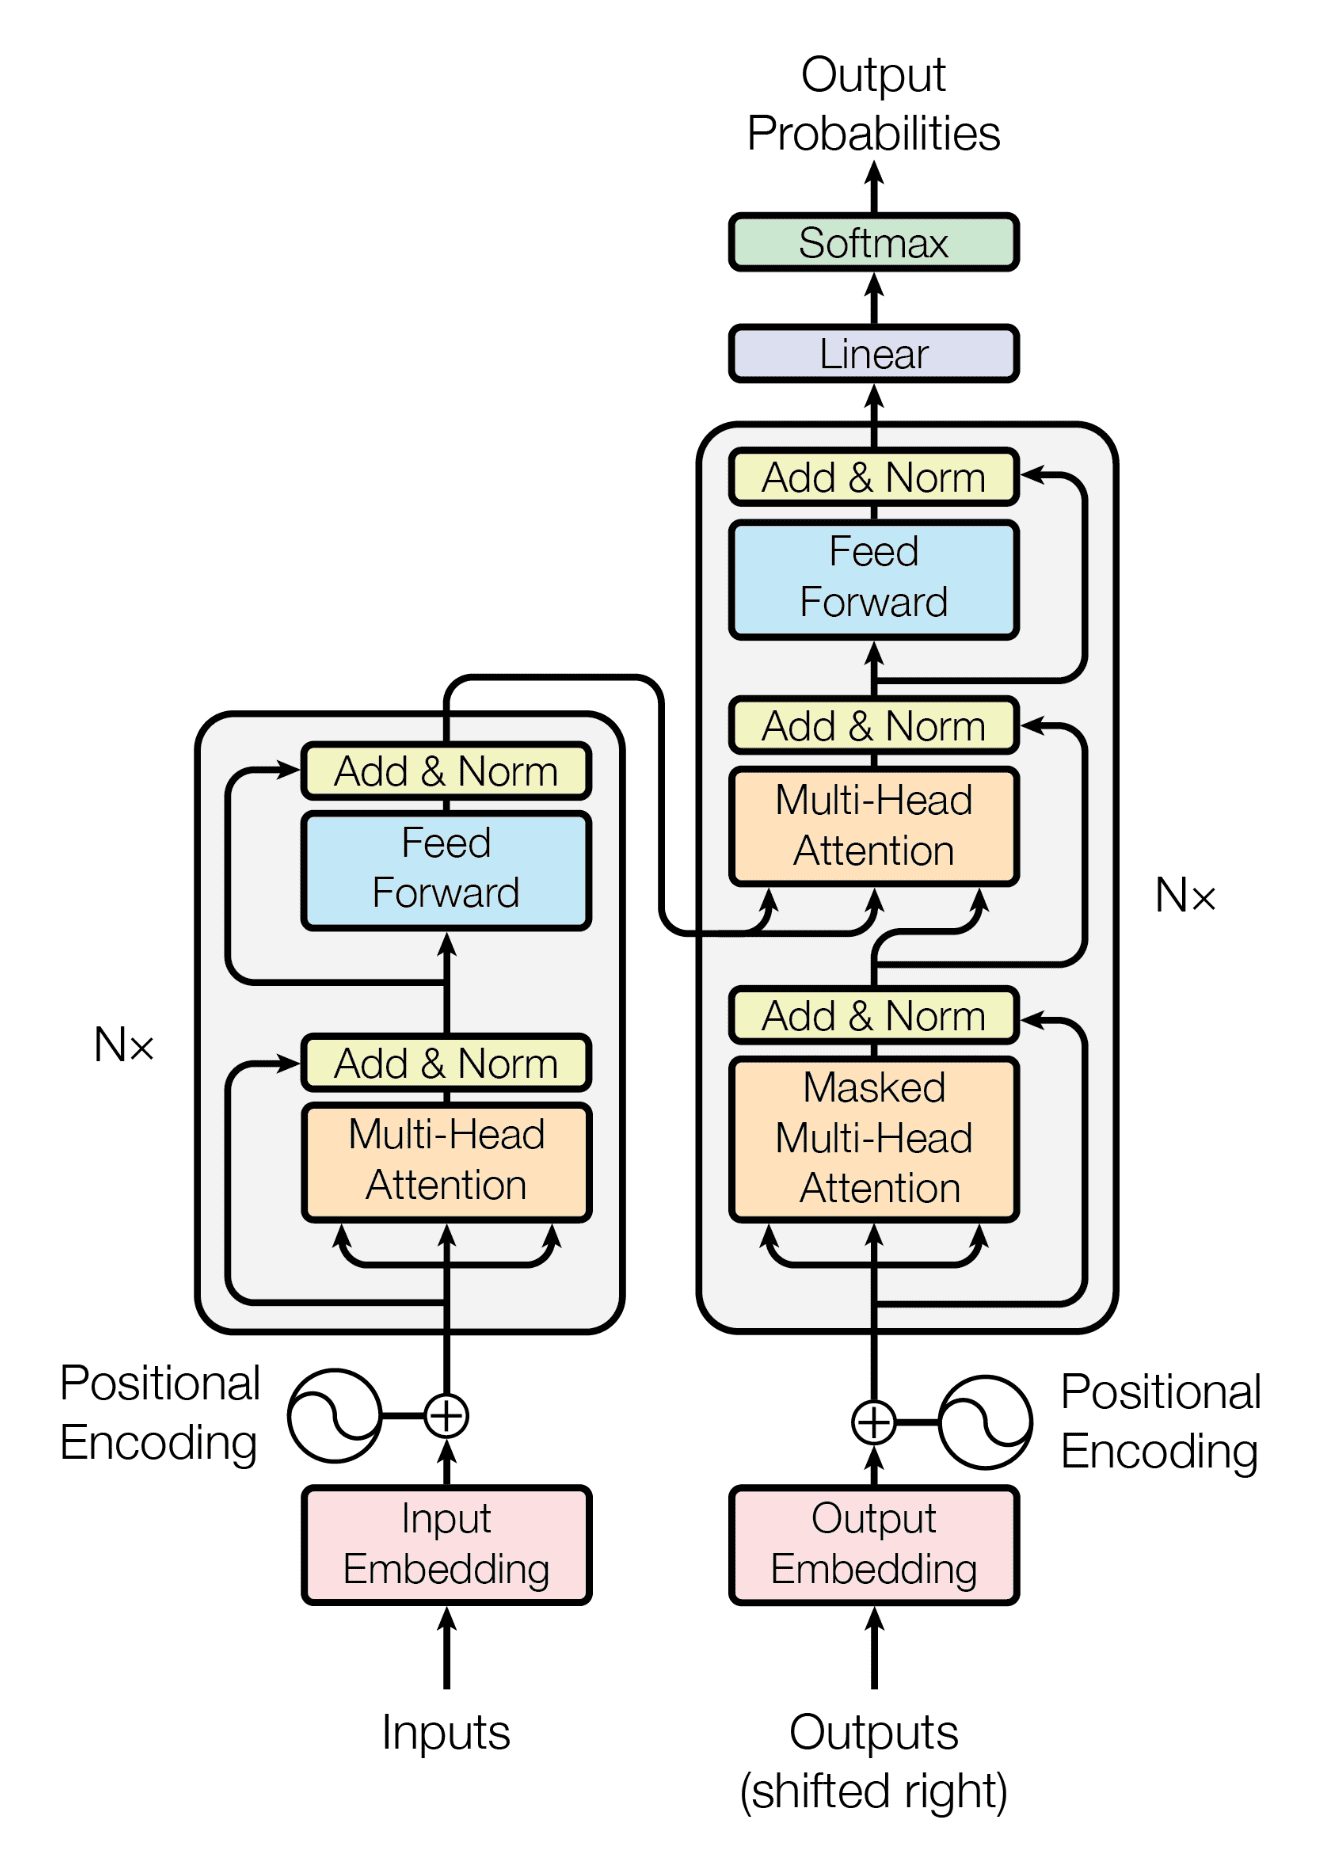
\includegraphics[height=0.8\textheight]{figs/transformer_arch.png}
\end{column}
\begin{column}{0.58\textwidth}
\vspace{10pt}
\begin{itemize}\setlength{\itemsep}{6pt}
  \item The architecture from \href{https://arxiv.org/abs/1706.03762}{\emph{Attention Is All You Need}} (Vaswani et al., 2017). GPT-style LLMs keep only the right half, the \textbf{decoder}: $N$ identical layers of attention + feed-forward, stacked.
  \item Look at the two ends: \textbf{embeddings} go in at the bottom; \textbf{Linear + Softmax} over the vocabulary comes out at the top. Those are the parts we care about today.
\end{itemize}
\vspace{4pt}
\keybox{\textbf{For today, the middle is a black box} $f_\theta$: a big differentiable function from the tokens so far to a vector $h_t$, trained by gradient descent. The course opens the box later (attention, Transformers).}
\end{column}
\end{columns}
\end{frame}

\begin{frame}{Inside the network (just enough for today)}
\begin{columns}[T]
\begin{column}{0.56\textwidth}
\begin{itemize}\setlength{\itemsep}{3pt}
  \item A deep stack of layers: $h^{(\ell)} = f^{(\ell)}_\theta\big(h^{(\ell-1)}\big)$, \; $L = 32$ for Llama-3-8B.
  \item Each layer: attention (mix information \emph{across positions}) + feed-forward (transform each position).
  \item Position $t$ only sees positions $\le t$: no cheating when predicting $x_{t+1}$.
  \item \textbf{Training:} all positions in parallel, in one forward pass; that is what makes trillions of tokens feasible.
  \item \textbf{Generation:} one token at a time, each conditioned on the ones before. This is called \emc{autoregressive} generation.
\end{itemize}
\end{column}
\begin{column}{0.42\textwidth}
\centering
\begin{tikzpicture}[font=\scriptsize,>=Latex,scale=0.9,every node/.style={transform shape}]
  \foreach \i/\w in {1/The,2/hippo,3/ate,4/my,5/homework}{
    \node[draw,fill=softgray,rounded corners,minimum width=0.9cm,minimum height=0.45cm] (in\i) at (1.15*\i,0) {\w};
    \node[draw,fill=uvanavy!15,circle,inner sep=2pt] (h1\i) at (1.15*\i,1.15) {};
    \node[draw,fill=uvanavy!15,circle,inner sep=2pt] (hL\i) at (1.15*\i,2.75) {};
    \draw[->] (in\i) -- (h1\i);
    \draw[->,gray!70,dashed] (h1\i) -- (hL\i);
  }
  \node[draw,fill=uvanavy!30,rounded corners,minimum width=5.7cm,minimum height=0.42cm] at (3.45,0.72) {layer 1 (attention + feed-forward)};
  \node[fill=white,inner sep=1pt,text=midgray] at (3.45,1.95) {$\vdots$\quad layers $2,\dots,L-1$\quad$\vdots$};
  \node[draw,fill=uvanavy!30,rounded corners,minimum width=5.7cm,minimum height=0.42cm] at (3.45,2.32) {layer $L$ (attention + feed-forward)};
  \node[left=0.5mm of hL5,text=uvanavy] {$h_t$};
  \node[draw,fill=okgreen!15,draw=okgreen!70!black,rounded corners,minimum width=1.5cm,minimum height=0.4cm] (sm) at (5.75,3.55) {linear + softmax};
  \draw[->,thick] (hL5) -- (sm);
  \node[anchor=south east,text=uvaorange!85!black] at ([yshift=1.5mm]sm.north east) {$p(\text{next token})$:\; ``.'' 0.5,\; ``yesterday'' 0.2,\; \dots};
  \node[text=midgray,align=center,font=\tiny] at (2.0,3.3) {(in training, every position\\predicts its own next token)};
\end{tikzpicture}
\end{column}
\end{columns}
\vspace{-2pt}
\callback{neural networks \& deep learning}{A Transformer is ``just'' another architecture: layers, nonlinearities, residuals, a loss at the top, gradients flowing down. Details later in this course.}
\end{frame}

\begin{frame}{The output layer is multi-class logistic regression}
At position $t$ the network gives $h_t\in\mathbb{R}^d$. Then
\[
  \underbrace{z_t = W_{\text{out}}\,h_t + b}_{\text{logits: one score per token}}\in\mathbb{R}^{|V|},
  \qquad
  p_t(i) = \frac{\exp(z_{t,i})}{\sum_{j=1}^{|V|}\exp(z_{t,j})}
\]
\begin{center}
\begin{tikzpicture}[font=\small,>=Latex]
  \matrix[matrix of nodes,left delimiter={[},right delimiter={]},row sep=0pt,nodes={inner sep=2pt}] (Z) at (0,0) {1.3\\5.1\\2.2\\0.7\\1.1\\};
  \node[left=5mm of Z-1-1,text=okgreen!70!black] {apple}; \node[left=5mm of Z-2-1,text=badred] {cake}; \node[left=5mm of Z-3-1,text=uvaorange!80!black] {banana};
  \node[left=5mm of Z-4-1] {$\dots$}; \node[left=5mm of Z-5-1] {$\dots$};
  \node[above=1mm of Z] {scores $z_t$};
  \node[draw,rounded corners,fill=softgray,minimum height=1.7cm,right=12mm of Z,align=center] (S) {softmax\\[3pt]$\dfrac{e^{z_i}}{\sum_j e^{z_j}}$};
  \matrix[matrix of nodes,left delimiter={[},right delimiter={]},row sep=0pt,nodes={inner sep=2pt},right=12mm of S] (P) {0.02\\0.90\\0.05\\0.01\\0.02\\};
  \node[above=1mm of P] {probabilities $p_t$};
  \draw[->,thick] (Z) -- (S); \draw[->,thick] (S) -- (P);
  \node[below=1mm of S,font=\scriptsize] {``I eat the \_\_\_''};
\end{tikzpicture}
\end{center}
\callback{logistic regression}{$p(y{=}1\mid x)=\sigma(w^\top x+b)$ is the 2-class case; softmax is its $K$-class generalization. Here the features are $h_t$ and $K=|V|\approx 100{,}000$. Nothing else is new.}
\end{frame}

\begin{frame}{Pretraining in one picture}
\begin{center}
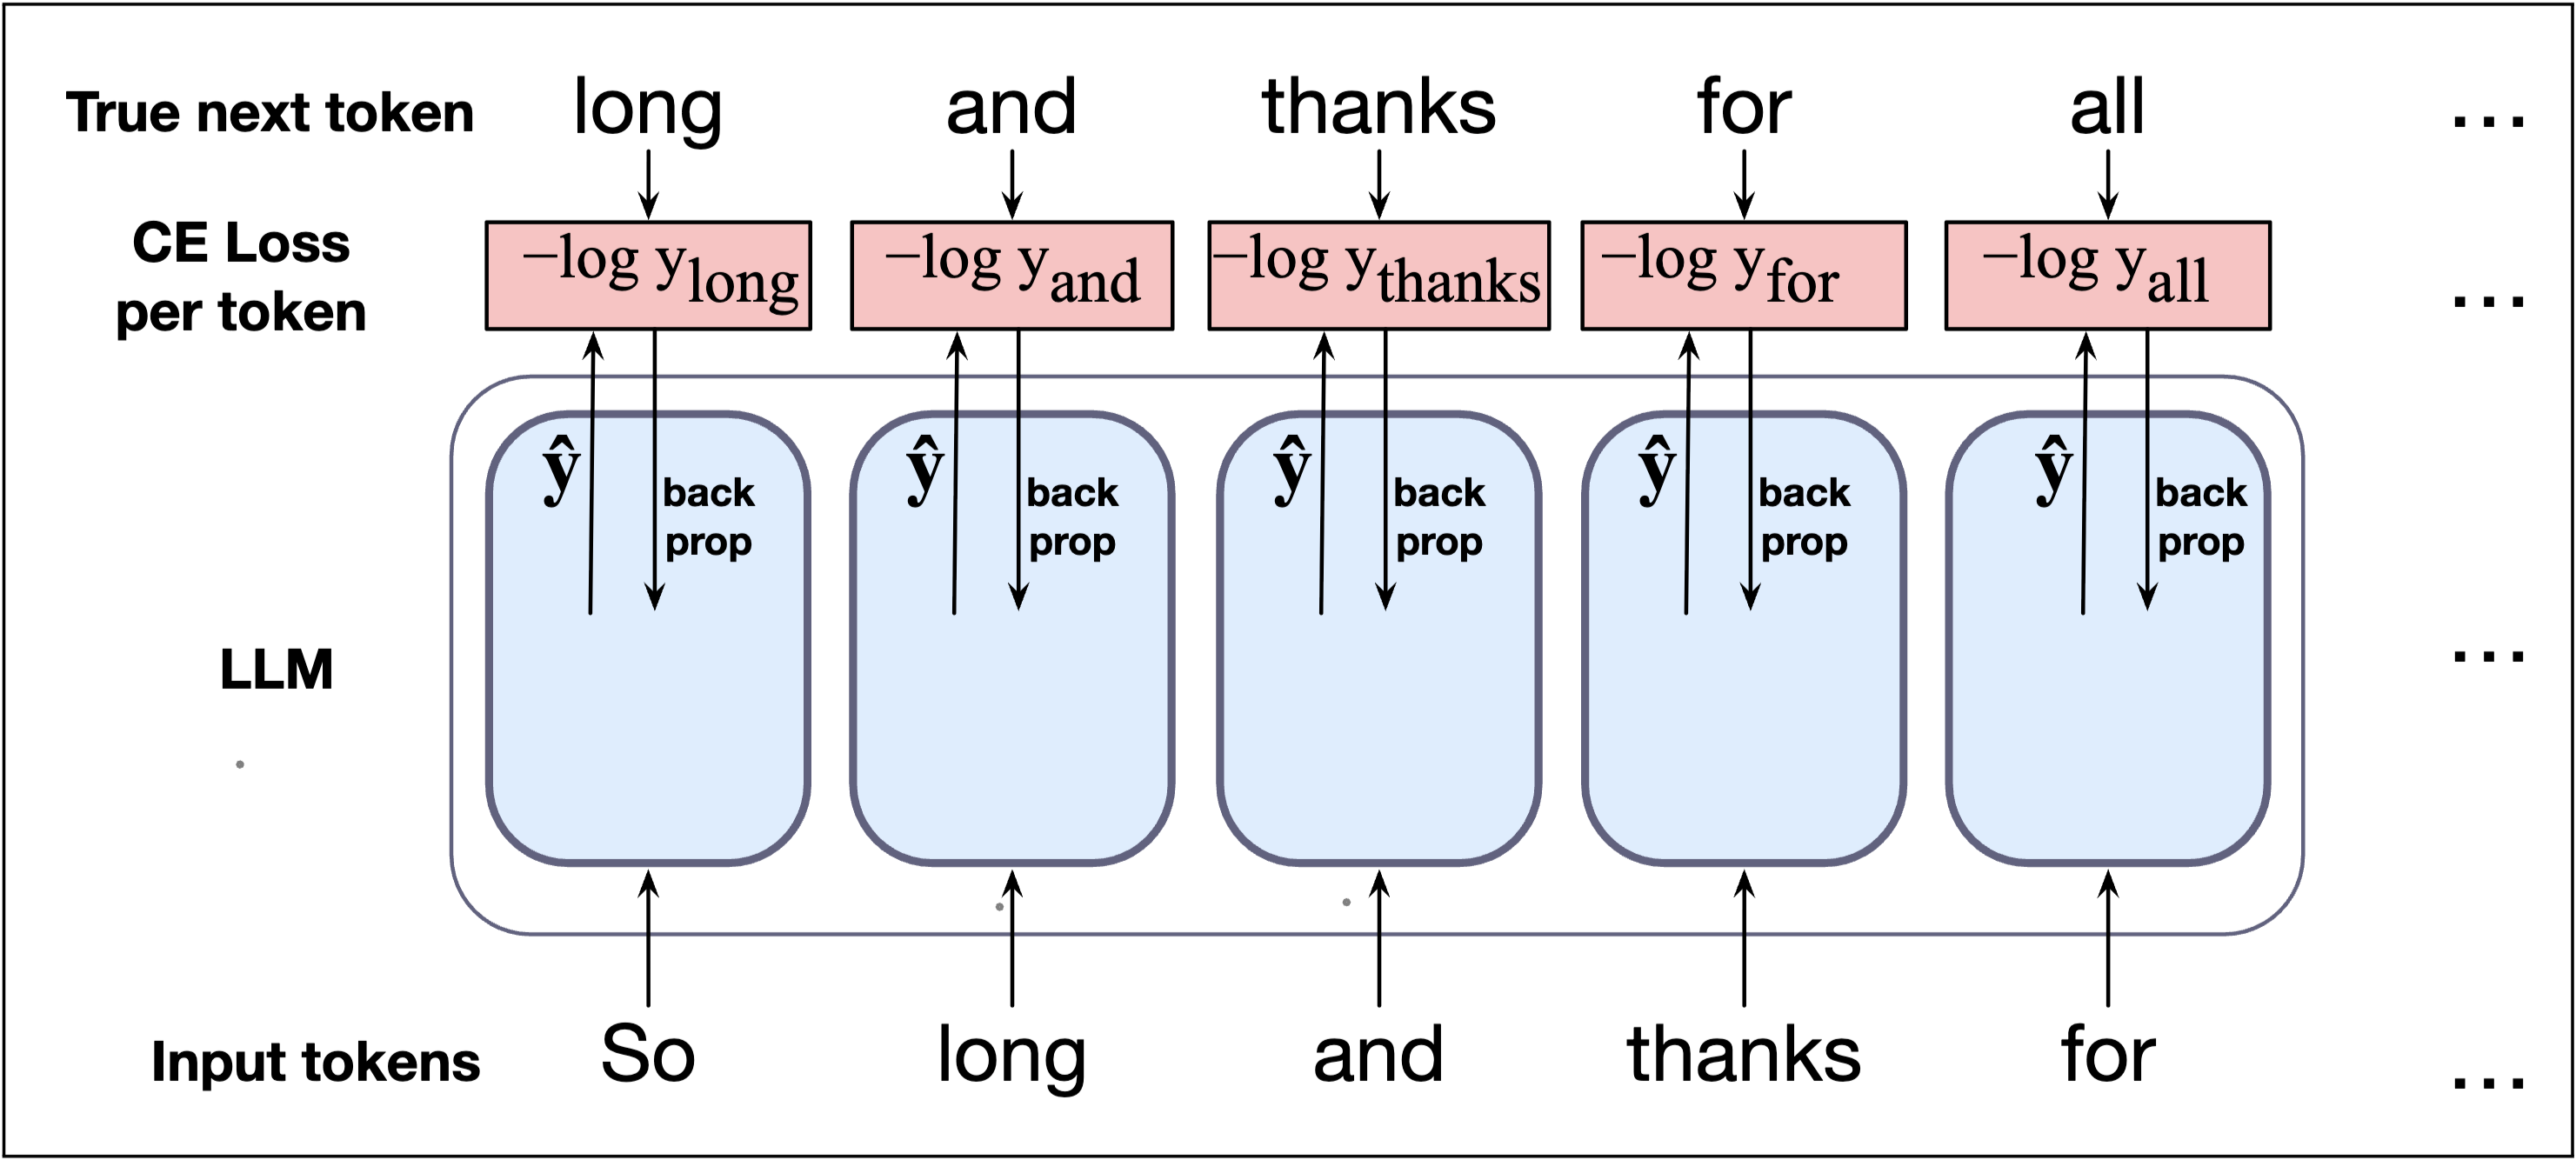
\includegraphics[width=0.74\textwidth]{figs/slp3_pretraining.png}
\end{center}
\vspace{-4pt}
\begin{itemize}\setlength{\itemsep}{2pt}
  \item Every position is a classification problem: the model outputs $\hat{y}$, a distribution over all possible next tokens.
  \item Loss at that position: the \textbf{negative log-likelihood (NLL)} of the \emc{true} next token, $-\log \hat{y}_{\text{true}}$. Average over the batch, backpropagate, update every weight (embeddings included).
\end{itemize}
\vspace{2pt}
{\scriptsize\color{midgray} Figure: Jurafsky \& Martin, \emph{Speech and Language Processing}, 3rd ed.}
\end{frame}

\begin{frame}{Training = cross-entropy = maximum likelihood on the corpus}
\textbf{Pretraining loss} (GPT-style, ``causal'' language modeling):
\[
  \mathcal{L}(\theta) = -\frac{1}{N}\sum_{t=1}^{N} \log p_\theta\big(x_t \mid x_{<t}\big)
\]
\begin{center}
\begin{tikzpicture}[font=\small,>=Latex]
  \foreach \i/\w in {1/The,2/hippo,3/ate,4/my,5/homework}{
    \node[draw,fill=softgray,rounded corners,minimum width=1.3cm,minimum height=0.55cm] (w\i) at (2.5*\i,0) {\w};
  }
  \foreach \i/\lab/\p/\l/\dy in {1/{p(\text{hippo}\mid\text{The})}/0.001/6.9/0,2/{p(\text{ate}\mid\text{The hippo})}/0.30/1.2/11,3/{p(\text{my}\mid\text{The hippo ate})}/0.08/2.5/0,4/{p(\text{homework}\mid\text{The hippo ate my})}/0.02/3.9/11}{
    \pgfmathtruncatemacro{\j}{\i+1}
    \draw[->,uvanavy,thick] (w\i.north) to[bend left=35] node[above=\dy pt,font=\scriptsize,fill=white,inner sep=1pt] {$\lab{=}\p$} (w\j.north);
    \node[below=3pt of w\j,font=\scriptsize,text=badred] {$-\log p = \l$};
  }
\end{tikzpicture}
\end{center}
\vspace{-2pt}
\begin{itemize}\setlength{\itemsep}{3pt}
  \item Each probability is conditioned on the \emc{whole prefix} $x_{<t}$, not just the previous word. Target at each position = the \textbf{actual next token}; loss = its NLL; average over positions.
  \item \textbf{Self-supervised}: the labels are free, the next word is already in the text. Minimized by \textbf{SGD (Adam)} + backprop.
\end{itemize}
\callback{MLE}{max $\prod_t p_\theta(x_t\mid x_{<t})$ $\Leftrightarrow$ min $-\sum_t\log p_\theta(x_t\mid x_{<t})$. Pretraining \emph{is} maximum likelihood.}
\end{frame}

\begin{frame}{Why does predicting the next word teach so much?}
Minimizing one loss on trillions of words forces the model to pick up every regularity that helps predict the next token:
\vspace{4pt}
\begin{center}\small
\renewcommand{\arraystretch}{1.3}
\begin{tabular}{@{}l l@{}}
\toprule
\textbf{to fill the blank it must learn \dots} & \textbf{example}\\
\midrule
grammar & In my free time, I like to \{\green{run}, \red{banana}\}\\
lexical semantics & At the zoo we saw giraffes, lions, and \{\green{zebras}, \red{spoon}\}\\
world knowledge & The capital of Denmark is \{\green{Copenhagen}, \red{London}\}\\
sentiment & Edge of my seat the whole time. The movie was \{\green{good}, \red{bad}\}\\
translation & The word for ``pretty'' in Spanish is \{\green{bonita}, \red{hola}\}\\
arithmetic & $3 + 8 + 4 = $ \{\green{15}, \red{11}\}\\
\bottomrule
\end{tabular}
\end{center}
\vspace{4pt}
\keybox{\textbf{Pretraining is implicit multi-task learning.} Nobody wrote a sentiment loss or a translation loss; the next-token loss already contains all of them.}
\end{frame}

\begin{frame}{Scale: more of everything, predictably better}
\begin{columns}[T]
\begin{column}{0.42\textwidth}
\begin{itemize}\setlength{\itemsep}{6pt}
  \item \textbf{Data:} Llama-3 saw $\sim$15 trillion tokens.
  \item \textbf{Parameters:} 0.1B (2018) $\to$ 175B (2020) $\to$ 405B (2024).
  \item \textbf{Compute:} thousands of GPUs for months.
  \item \textbf{Scaling laws} (\href{https://arxiv.org/abs/2001.08361}{Kaplan et al., 2020}): test loss falls as a \textbf{power law} in each factor: straight lines on log-log axes.
\end{itemize}
\end{column}
\begin{column}{0.56\textwidth}
\centering
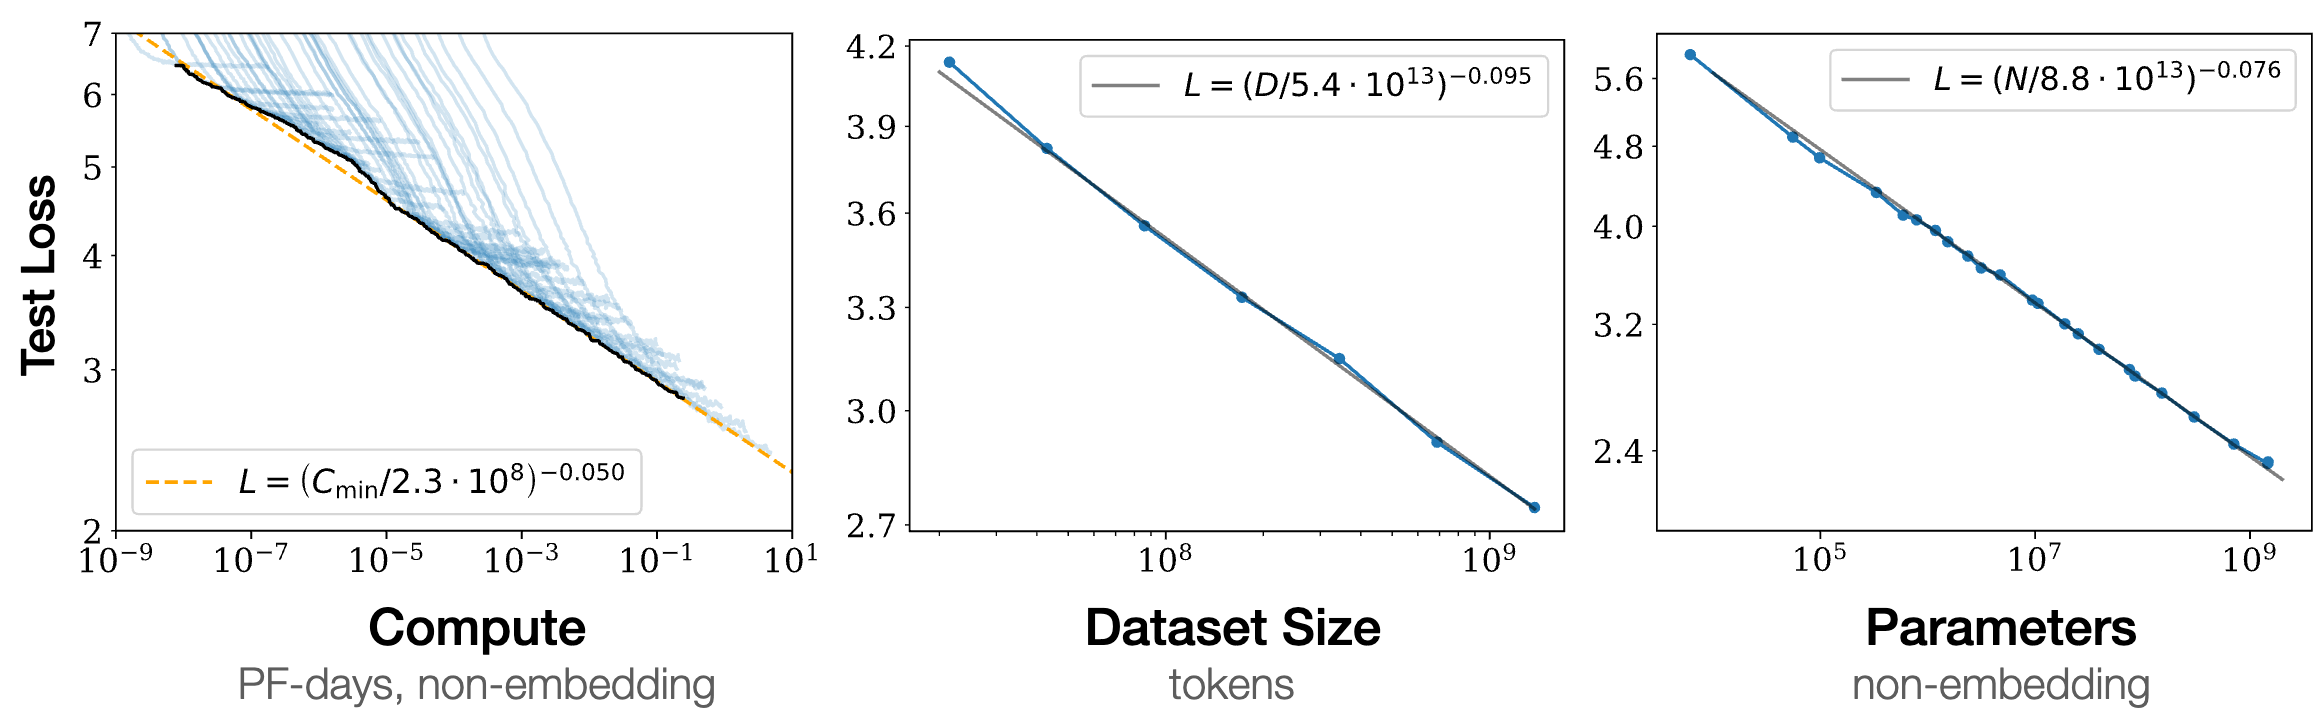
\includegraphics[width=\textwidth]{figs/scaling_laws.png}\\[2pt]
\scriptsize Test loss vs.\ training compute (in PF-days: $10^{15}$ floating-point ops per second, sustained for a day), dataset size (tokens), and parameters.
\end{column}
\end{columns}
\vspace{6pt}
\callback{bias--variance}{Test loss keeps improving with more data \emph{and} more parameters; these models are nowhere near the regime where extra capacity hurts.}
\end{frame}

\begin{frame}{Emergent abilities: some skills appear only at scale}
\begin{columns}[T]
\begin{column}{0.58\textwidth}
\centering
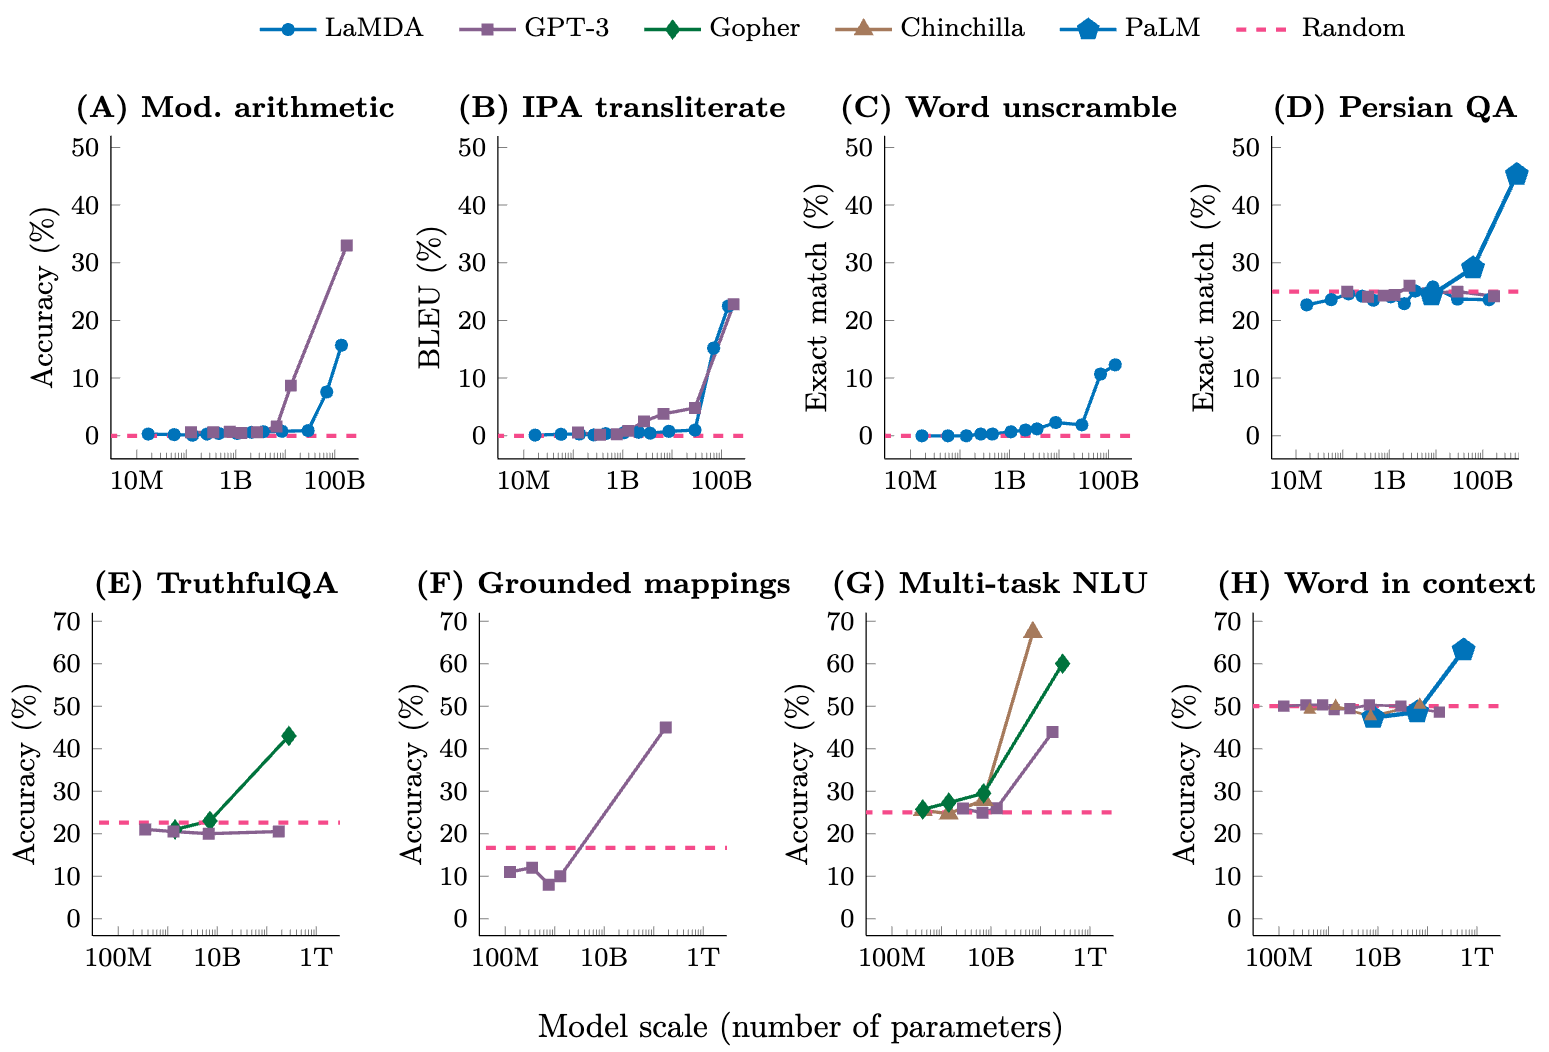
\includegraphics[width=\textwidth]{figs/emergent_plot.png}
\end{column}
\begin{column}{0.4\textwidth}
\begin{itemize}\setlength{\itemsep}{6pt}
  \item Few-shot accuracy on arithmetic, word unscrambling, multi-task understanding, \dots
  \item Stays at \textbf{chance} until a size threshold, then jumps --- not predictable from smaller models.
  \item The same recipe at larger scale gave GPT-3 the ability in Part 3: learning from examples in the prompt.
\end{itemize}
\end{column}
\end{columns}
\end{frame}

\begin{frame}{Decoding: from a probability distribution to text}
\begin{columns}[T]
\begin{column}{0.5\textwidth}
Loop: compute $p_t$ $\to$ pick a token $x_t$ $\to$ append $\to$ repeat until \texttt{<EOS>}.
\begin{itemize}\setlength{\itemsep}{4pt}
  \item \textbf{Greedy:} $x_t = \arg\max_i p_t(i)$. Deterministic; bland, repetitive.
  \item \textbf{Sampling:} $x_t \sim p_t$. Diverse; may pick nonsense from the tail.
  \item \textbf{Temperature $\tau$:} $p^{(\tau)}_t(i) \propto \exp(z_{t,i}/\tau)$ --- $\tau\to 0$ greedy, $\tau\uparrow$ flatter.
  \item \textbf{Top-$k$ / top-$p$:} sample only from the most likely tokens.
\end{itemize}
\end{column}
\begin{column}{0.48\textwidth}
\centering
\begin{tikzpicture}
\begin{groupplot}[group style={group size=3 by 1,horizontal sep=0.25cm},width=0.36\textwidth,height=3.2cm,
  ybar,/pgf/bar width=5pt,ymin=0,ymax=1,xtick=data,symbolic x coords={cake,pie,apple,banana,rock},
  xticklabel style={rotate=60,anchor=east,font=\tiny},ytick={0,0.5,1},yticklabel style={font=\tiny},
  title style={font=\scriptsize,yshift=-4pt},enlarge x limits=0.2]
\nextgroupplot[title={$\tau=0.5$}]
\addplot[fill=uvanavy!60,draw=uvanavy] coordinates {(cake,0.831) (pie,0.112) (apple,0.041) (banana,0.015) (rock,0.0003)};
\nextgroupplot[title={$\tau=1$},yticklabels={}]
\addplot[fill=uvaorange!70,draw=uvaorange!80!black] coordinates {(cake,0.573) (pie,0.211) (apple,0.128) (banana,0.078) (rock,0.010)};
\nextgroupplot[title={$\tau=2$},yticklabels={}]
\addplot[fill=okgreen!60,draw=okgreen!70!black] coordinates {(cake,0.387) (pie,0.235) (apple,0.183) (banana,0.142) (rock,0.052)};
\end{groupplot}
\end{tikzpicture}\\
\scriptsize Same logits for ``I eat the \_\_\_'', three temperatures.
\end{column}
\end{columns}
\vspace{6pt}
\keybox{Why ChatGPT answers the same question differently each time --- and why ``sample several answers to one question'' is a key tool in Part 7.}
\end{frame}
